%------------------------------------------------------------------------------------
\newpage
\section{Теоретическая часть}
%------------------------------------------------------------------------------------
\subsection{OFDM модуляция}

Данный вид модуляции подразумевает передачу суммы нескольких гармоник
— поднесущих, частоты которых выбираются из условия ортогональности %(\ref{Dahlman2011-bk})
. В формуле~\ref{eq:ofdm_base}
представлено математическое описание OFDM сигнала:

%------------------------------------------------------------------------------------
% Equation
%------------------------------------------------------------------------------------
\begin{equation}
    Y_i = \sum_{n = 1}^{N} X_n e^{j 2 \Pi f_n t},
    \label{eq:ofdm_base}
\end{equation}
%------------------------------------------------------------------------------------

где $Y_i$ - OFDM отсчет, $N$ - количество поднесущих, $X_n$ - отсчет полезного сигнала,
$f_n$ - частота $n$-ой поднесущей.

Частоты поднесущих получаются из выражения (\ref{eq:subc_eq}):

%------------------------------------------------------------------------------------
% Equation
%------------------------------------------------------------------------------------
\begin{equation}
    f_n = n \Delta f,
    \label{eq:subc_eq}
\end{equation}
%------------------------------------------------------------------------------------

где $\Delta f$ - расстояние между поднесущими.

%------------------------------------------------------------------------------------
% Figure
%------------------------------------------------------------------------------------
\begin{figure}[h]
    \centering
    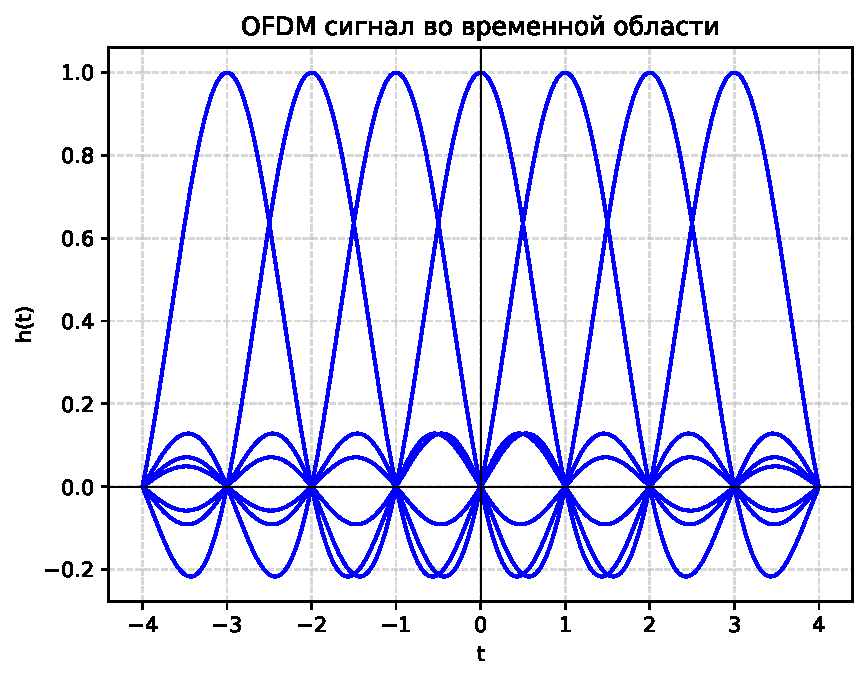
\includegraphics[width=0.8\textwidth]{images/1_ofdm_td.pdf}
    \caption{OFDM сигнал в частотной области}
    \label{fig:ofdm_fd}
\end{figure}
%------------------------------------------------------------------------------------

На рис.~\ref{fig:ofdm_fd} показан OFDM сигнал в частотной области, где отдельные несущие
не перекрываются из-за ортогональности.

При последовательной передаче высокоскоростного потока данных, как
правило, возникает проблема, связанная c тем, что период передачи символов
намного меньше, чем время задержки в канале %(\ref{Sesia2009-fj})
.
Это создает помехи в виде
символьной интерфененции, в ходе чего происходит наложение символов, которые можно устранить c помощью эквалайзинга.
В OFDM высокоскоростной поток символов данных сначала последовательно-
параллельным образом преобразуется для модуляции на $N$ параллельных
поднесущих (рис.~\ref{fig:ofdm_tx}). Это увеличивает период передачи символов на каждой
поднесущей так, что он становится значительно больше, чем временные
задержки в канале. После модуляции, сигнал поступает
на блок ОБПФ и на парралельно-последовательный преобразователь, на котором вводится циклический
префикс - введение избыточности в начале OFDM символа для борьбы с межсимвольной интерференцией.
Приемник устроен аналогично (рис.~\ref{})

%------------------------------------------------------------------------------------
% Figure
%------------------------------------------------------------------------------------
\begin{figure}[h]
    \centering
    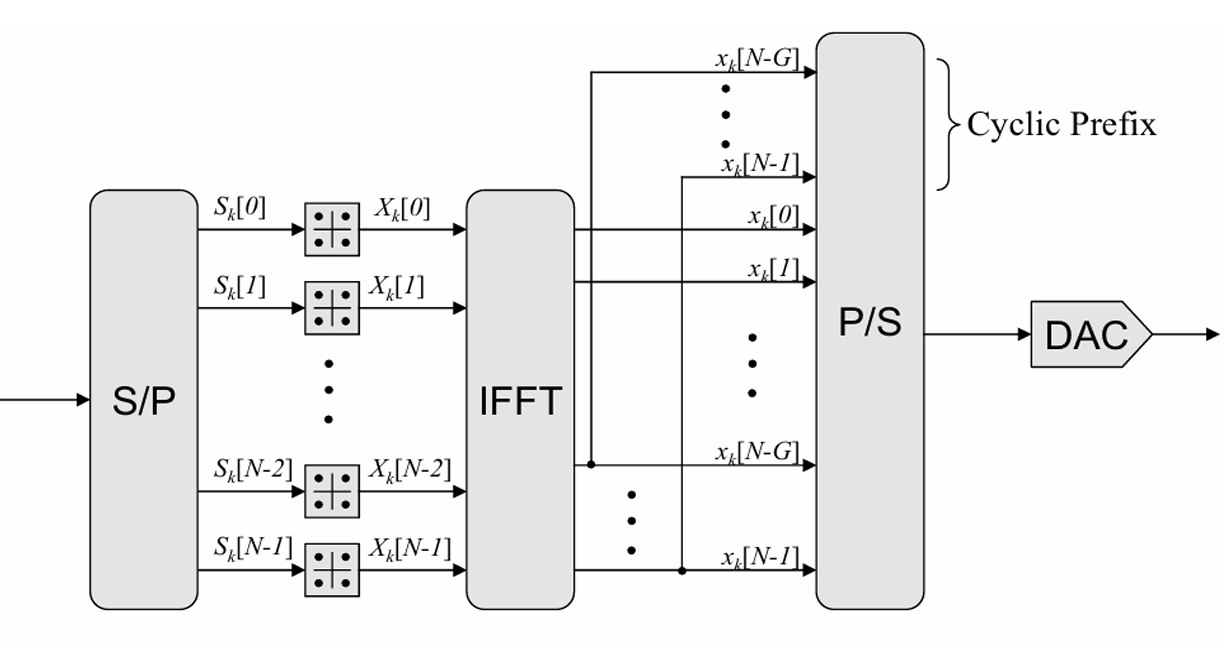
\includegraphics[width=0.8\textwidth]{images/1_ofdm_tx.png}
    \caption{Схема передатчика OFDM}
    \label{fig:ofdm_tx}
\end{figure}
%------------------------------------------------------------------------------------

%------------------------------------------------------------------------------------
% Figure
%------------------------------------------------------------------------------------
\begin{figure}[h]
    \centering
    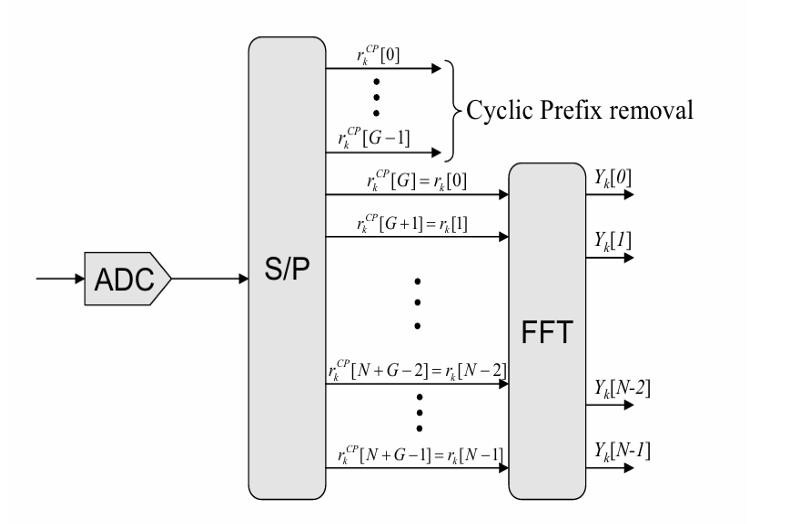
\includegraphics[width=0.8\textwidth]{images/1_ofdm_rx.png}
    \caption{Схема приемника OFDM}
    \label{fig:ofdm_rx}
\end{figure}
%------------------------------------------------------------------------------------


%------------------------------------------------------------------------------------
\subsection{Эффект Допплера}

Эффект Доплера возникает при наличии радиальной
скорости приемника или передатчика относительно друг друга (\ref{eq:dopp}). 

%------------------------------------------------------------------------------------
% Equation
%------------------------------------------------------------------------------------
\begin{equation}
    f_d = \frac{v f}{c} \cos \psi ,
    \label{eq:dopp}
\end{equation}
%------------------------------------------------------------------------------------

где $fd$ - доплеровское смещение частоты, $v$ - модуль относительной скорости между
премником и передатчиком, $f$ - частота сигнала, $\psi$ - угол между вектором скорости и
радиус вектором от приемника к передатчику (рис.~\ref{fig:doppler}).

%------------------------------------------------------------------------------------
% Figure
%------------------------------------------------------------------------------------
\begin{figure}[h]
    \centering
    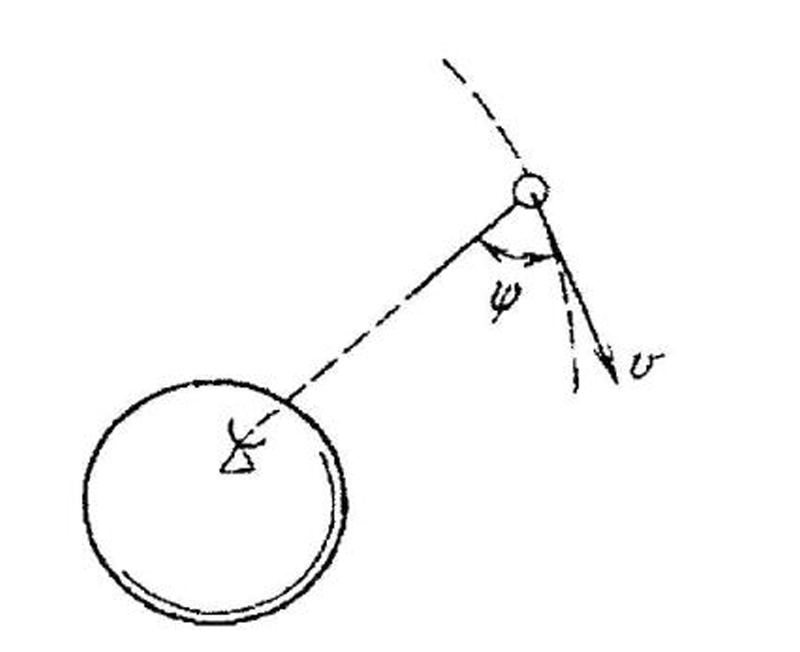
\includegraphics[width=0.8\textwidth]{images/1_doppler.png}
    \caption{Схема для расчета доплеровского смещения}
    \label{fig:doppler}
\end{figure}
%------------------------------------------------------------------------------------

В канале связи при наличии отражающих и рассеивающих обьектов возникает многолучевое
распространение радиосигнала. Эффект многолучевого распространения сигнала описывается
моделями канала, как детерминироваными (ray-tracing propagation models), так и стохастическими
(напр. модель Джейкса).
% Тут нужно сослаться на соответсвующую литературу

Если считать сигнал узкополосным, то эффект Доплера приводит к смещению спектра. В моделях
канала с многолучевым распространением (напр. модель Релея-Джейкса), вводится такое допущение
для OFDM сигнала, т.е. смещение действует на весь спектр вцелом. Но вследствии многолучевости,
отраженные сигналы приходят на приемник с разных углов и с разным смещением, тем самым достигается
эффект "размытия спектра". Такой подход позволяет достаточно просто учитывать и многолучевость,
и эффект Допплера (сдвиг и размытие).

Если такое допущение не принимать, т.е. считать сигнал широкополосным, то на каждую поднесущую
сигнала будет действовать разный сдвиг частоты, что приводит к интерференции между поднесущими (ICI).
Это можно представить следующим образом (\ref{eq:ofdm_dopp_full}):

%------------------------------------------------------------------------------------
% Equation
%------------------------------------------------------------------------------------
\begin{equation}
    Y_i = \sum_{n = 1}^{N} X_n e^{j 2 \Pi (f_n + f_c) (1 + \varepsilon ) t},
    \label{eq:ofdm_dopp_full}
\end{equation}
%------------------------------------------------------------------------------------

где $f_c$ - несущая частота сигнала, $\varepsilon = \frac{v}{c} \cos \psi$ - коэффициент доплеровского смещения.

Обычно, в спутниковых системах связи доплеровское смещение заранее известно, так как 
известны координаты и скорость спутника, поэтому можно предавать сигнал с учетом этого
смещения $Y^`_i = Y_i e^{- 2 j \Pi f_c \varepsilon}t$, тем самым избавляясь от этого эффекта.
В сетях наземной мобильной связи можно по специальным сигналам для оценки канала, которые передаются
на выделенных поднесущих, так называемые референсные сигналы, оценить смещение и отфильтровать его
на эквалайзере. Наконец, уход несущей частоты может исправить система фазовой автоподстойки частоты (ФАПЧ)
на приемнике. Исходя из этого, в дальнейших рассуждениях несущая частота сигнала не будет учитываться,
так как ее вклад в искажение сигнала зачастую учитывается.

Таким образом, в данной работе влияние доплера сводится к следующему выражению (\ref{eq:ofdm_dopp_real}):
%------------------------------------------------------------------------------------
% Equation
%------------------------------------------------------------------------------------
\begin{equation}
    Y_i = \sum_{n = 1}^{N} X_n e^{j 2 \Pi f_n (1 + \varepsilon ) t},
    \label{eq:ofdm_dopp_real}
\end{equation}
%------------------------------------------------------------------------------------

%------------------------------------------------------------------------------------
\subsection{Оценка ICI и BER}



%------------------------------------------------------------------------------------
\subsection{Модель системы передачи данных}

Модель передачи данных для исселедования зависимостей ICI И BER от доплеровского расширения
спектра должна включать в себя прередатчик (рис.~\ref{fig:ofdm_tx}), канал связи с аддитивным белым
гауссовым шумом (AWGN) и приемник (рис.~\ref{fig:ofdm_rx}). Моделирование расширения спектра будет
реализовано с помощью множителей, которые будут применяться к каждой поднесущей сигнала в частотной 
области, т.е. до применения ОБПФ (рис.~\ref{fig:ofdm_scheme}):

%------------------------------------------------------------------------------------
% Figure
%------------------------------------------------------------------------------------
\begin{figure}[h]
    \centering
    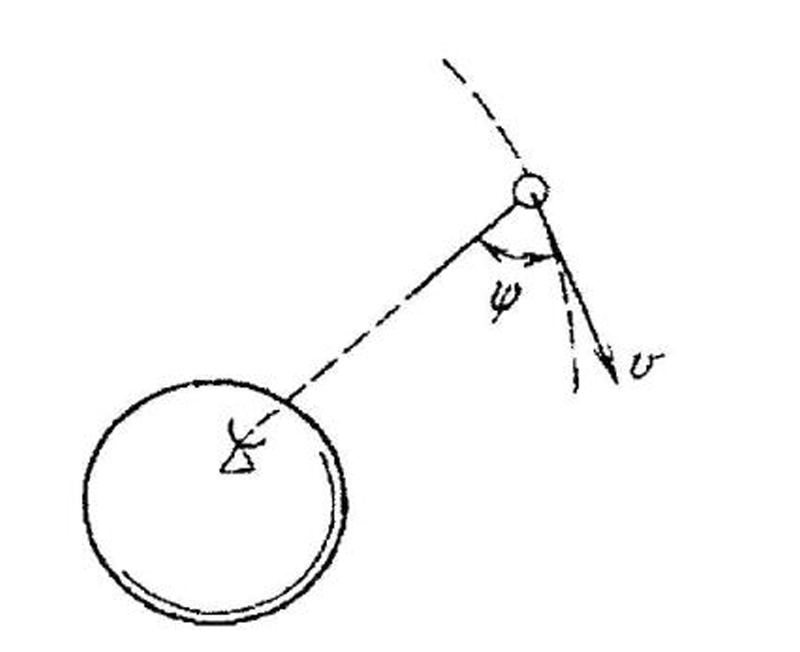
\includegraphics[width=0.8\textwidth]{images/1_doppler.png}
    \caption{Схема модели передачи OFDM сигнала с учетом доплеровского масштабирования спектра}
    \label{fig:ofdm_scheme}
\end{figure}
%------------------------------------------------------------------------------------

